\chapter{پیاده سازی عملی پروژه کارآموزی}
در این فصل به پیاده سازی عملی این پروژه و چالش های آن اشاره خواهد شد. با توجه به نتیجه گیری هایی که در مطالعات نظری فصل قبل بدست آمد تصمیم بر این شد که معماری ای-برانچفرمر\LTRfootnote{E-Branchformer}
با استفاده ابزار 
یی-اس-پی نت
و دادگان 
\verb|Voice Common|
برای زبان فارسی آموزش داده شود. مدل حاصل اگر نتایج خوبی داشته باشد می تواند بجای مدل فعلی نرم افزار نویسا شرکت عصر گویش پرداز استفاده شود.


برای پیاده سازی عملی پروژه بر اساس دستور مسئول کارآموزی باید مراحل زیر انجام شود.
\begin{enumerate}

  \item ارئه گزارش از مباحث تئوری پروژه در جلسه آزمایشگاه دکتر صامتی

  \item فراگیری ابزار مورد نیاز پروژه

  \item آموزش مدل بر روی دادگان

  \item بررسی خروجی و رفع ایرادات

  \item فراگیری مباحث مورد نیاز برای پیاده سازی بر روی سرور

  \item پیاده سازی بر روی سرور

  \item مستندسازی و ارائه خروجی
  

\end{enumerate}

در ادامه این فصل هر یک از مراحل پیاده سازی عملی پروژه توضیح داده خواهد شد.

\section{ارائه مباحث نظری پروژه در جلسه آزمایشگاه}

بعد از انجام مطالعات نظری که در فصل قبل بیان شد گزارشی از اقدامات انجام شده و مباحث آموخته شده آماده شد و در جلسه آزماشگاه دکتر صامتی خدمت خود دکتر و دستیاران ایشان ارائه شد. بعد از ارائه، از نظرات ایشان و دیگر اعضای آزمایشگاه برای ادامه کار استفاده شد.
طبق نظر دکتر باید خروجی مدل بر روی پایگاه داده خود شرکت بررسی شود تا عملکرد آن را با مدل های قبلی شرکت مقایسه کرد.
همچنین با توجه به اینکه در بازشناسی گفتار به دو مدل صوت شنانسی\LTRfootnote{Acoustic} و زبانی برای دریافت خروجی نیاز می باشد؛ باید مدل زبانی بر روی دادگان پایگاه داده ناب آموزش داده شود تا مدل زبانی قوی برای این پروژه تهیه شود.


پیکره متنی ناب یکی از پروژه های شرکت عصر گویش پرداز می‌باشد که در آن 225892925	
جمله فارسی موجود می‌باشد که این جملات شامل متن های رسمی،غیر رسمی و حتی انواع اشعار فارسی می باشد. حجم زیاد داده های این مدل و تنوع خوب آن، این پایگاه داده منبع باز را به مرجع کاملی برای زبان فارسی کرده است.\cite{sabouri2022naab}

\section{فراگیری ابزار مورد نیاز پروژه}
یکی از طولانی ترین و سخت ترین بخش های پروژه در یادگیری جعبه ابزار\LTRfootnote{Toolkit}
مورد نیاز این پروژه بود. بعد از مطالعات تئوری نظر بر این شد که از ابزار
یی-اس-پی نت\LTRfootnote{ESPnet}
در این پروژه استفاده شود.
یی-اس-پی نت
ابزاری بسیار قدرتمند در پردازش گفتار است و همه تسک های پردازش گفتار را به خوبی پوشش می دهد. این ابزار اخیرا بسیار توسط محققین استفاده میشود و پیاده سازی پردازش گفتار به این ابزار انجام می دهند.
با توجه به این که در مقاله ای-برانچفرمر این معماری در 
یی-اس-پی نت
پیاده سازی شده است پس یادگیری این ابزار کار آمد اجتناب ناپذیر می‌باشد.

یی-اس-پی نت
عمدتاً بر روی بازشناسی خودکار گفتار سرتاسر
\LTRfootnote{End to End}
تمرکز دارد و از ابزارهای شبکه عصبی پویا پرکاربرد، 
\verb|Chainer|
و 
\verb|PyTorch|
، به عنوان یک موتور یادگیری عمیق اصلی استفاده می‌کند.
یی-اس-پی نت
همچنین از سبک جعبه ابزار 
\verb|ASR Kaldi|
برای پردازش داده ها، استخراج ویژگی/قالب، و دستور العمل ها پیروی می کند تا یک راه اندازی کامل برای تشخیص گفتار و سایر آزمایش های پردازش گفتار ارائه دهد. 
یی-اس-پی نت
به طور کامل از مزایای دو پیاده سازی 
\verb|ASR|
سر به سر بر اساس طبقه بندی زمانی اتصالگرا 
\LTRfootnote{CTC: Connectionist Temporal Classification}
و شبکه انکدر-دیکدر مبتنی بر 
توجه\LTRfootnote{Attention}
استفاده می کند. روش‌های مبتنی بر 
توجه
از مکانیزم توجه برای انجام هم‌ترازی بین فریم‌های صوتی و نمادهای شناسایی استفاده می‌کنند، در حالی که 
\verb|CTC|
از مفروضات مارکوف برای حل مؤثر مسائل متوالی توسط برنامه‌نویسی پویا استفاده می‌کند. 
یی-اس-پی نت
ترکیبی 
\texttt{\raggedright CTC}
و
\texttt{\raggedright Attention}
سر به سر
را اتخاذ می کند که به طور مؤثر از مزایای هر دو معماری در آموزش و رمزگشایی استفاده می کند. در طول آموزش، از چارچوب یادگیری چندهدفه برای بهبود استحکام در ترازهای نامنظم و دستیابی به همگرایی سریع استفاده می‌شود. در طول دیکد کردن، رمزگشایی مشترک را با ترکیب امتیازات مبتنی بر توجه و 
\verb|CTC|
در یک الگوریتم جستجوی پرتوی یک‌گذر انجام می‌دهد تا ترازهای نامنظم را حذف کند.\cite{watanabe2018espnet}
\LTRfootnote{\url{https://github.com/espnet/espnet}}

یکی از بزرگ ترین مشکلات این ابزار نبود مستندات کافی برای آموزش کار با این ابزار می‌باشد. با توجه به اینکه هیچ کس در شرکت به این ابزار تسلط نداشت و آموزشی هم در اینترنت برای کار با این مدل موجود نبود؛ فراگیری کار با این ابزار بسیار سخت و زمان بر بود.
برای یادگیری کا با ابزار من جبور شدم که تمام کد های موجود در این صفحه این ابزار را مطالعه کنم. باگ ها پیام های مناسبی را نمایش نمی‌دادند و دیباگ کردن حل مشکلات با این ابزار بسیار زمان بر بود.

همچنین وابستگی این ابزار به ابزار 
\verb|Kaldi|
من را وادار کرد که مستندات این ابزار را هم مطالعه کنم تا بتوانم مدل خود را آموزش دهم.
این ابزار سنگین است و نصب آن معمولا 10 الی 15 دقیقه طول می‌کشد و با توجه اینکه این ابزار بر روی
گوگل کلب\LTRfootnote{Google Colab}
نصب نمی‌باشد؛ برای هربار استفاده از کد باید یک بار آن را نصب کنیم که فرآینده آموزش مدل را بسیار طولانی می‌کند.
با توجه به این مشکلات حجم زیاد دادگان تصمیم بر این شد که من
یی-اس-پی نت
را بر روی یکی از سرور های شرکت نصب کنم و آموزش را با آن انجام دهم.
اینکار زمان نصب و دانلود داده ها را نسبت به گوگل کلب بسیار کمتر می‌کند اما کار با این ابزار یکی از چالش هایی بود که من همچنان باید با آن در طول این کارآموزی دست و پنجه نرم می‌کردم.

در نهایت بعد از دو هفته تلاش من موفق شدم که مدل صوت شنانسی را بر روی دادگان کامن ویس
آموزش دهم.
برای آموزش مدل های بازشناسی گفتار در ابزار
یی-اس-پی نت
اقدامات زیر انجام شد.

\begin{enumerate}

  \item دانلود داده ها

  \item انجام مراحل پیش پردازش (حذف داده های بلند و کوتاه، تبدیل داده ها به فرمت کلدی، تغییر فرمت داده به  \texttt{WAV} و ...)

  \item افزایش داده ها برای جلوگیری از اورفیت شدن (افزایش و کاهش سرعت گفتار و اضافه کردن نویز به داده های صوتی)

  \item ایجاد توکن لیست\LTRfootnote{Token List} با استفاده از داده ها متنی

  \item ایجاد پیکربندی\LTRfootnote{Config} مدل (مشخص کردن معماری، مشخص کردن انجام مینی-بچ\LTRfootnote{Mini-Batch} ها با استفاده واریانس داده ها و ... )

  \item آموزش مدل (این مرحله دو روز به طول انجامید)

  \item دیکد کردن مدل بر روی دادگان آزمایش کامن ویس

  \item محاسبه متریک های خطا

\end{enumerate}

\section{آموزش مدل بر روی دادگان}

کدهای پیاده سازی اولیه موجود می‌باشد البته این کد ها در گوگل کلب زده شده اند ولی بر روی سرور شرکت اجرا شده اند. جزیئات معماری و هایپر پارامتر های آن در کد زیر قابل دریافت است \LTRfootnote{ \url{https://colab.research.google.com/drive/15FfGd7uUQ-m8NUEn-wJLvjVJ62kQ9_T6?usp=sharing}}

یکی دیگر از مشکلاتی که با آن در این دوره درگیر شدم کمبود حافظه واحد پردازش گرافیکی بود. به علت بزرگ بودن مدل و زیاد بودن حجم داده سرور شرکت قادر نبود مدل را آموزش دهد تا زمانی که در مرحله 5 آموزش مدل مقدار بچ سایز ها را کوچک کردیم تا بتوانیم مدل را آموزش دهیم. این کار باعث شد روند آموزش پایدار شود اما زمان مورد نیاز برای آموزش مدل را افزایش داد به طوری که یک روز برای آموزش و نصف روز برای دیکد کردن مدل بر روی داده های تست استفاده شد.

\begin{figure}[h]
		\centering % <-- added
		\begin{subfigure}{0.5\textwidth}
			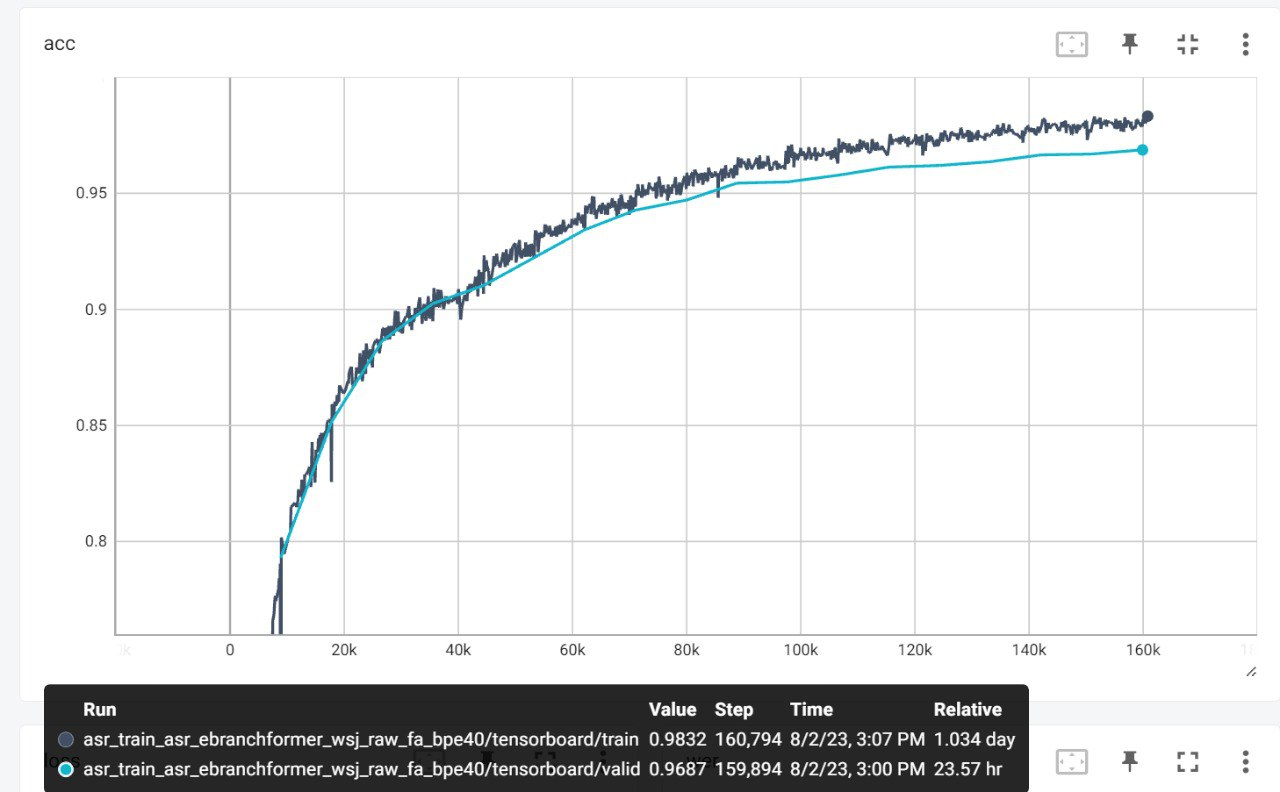
\includegraphics[width=1.1\linewidth, 
                    height=0.25\textheight]
                    {Images/Chapter3/train2.jpg}
			\caption{دقت مدل}
			\label{Acc}
		\end{subfigure}\hfil % <-- added
		\begin{subfigure}{0.5\textwidth}
			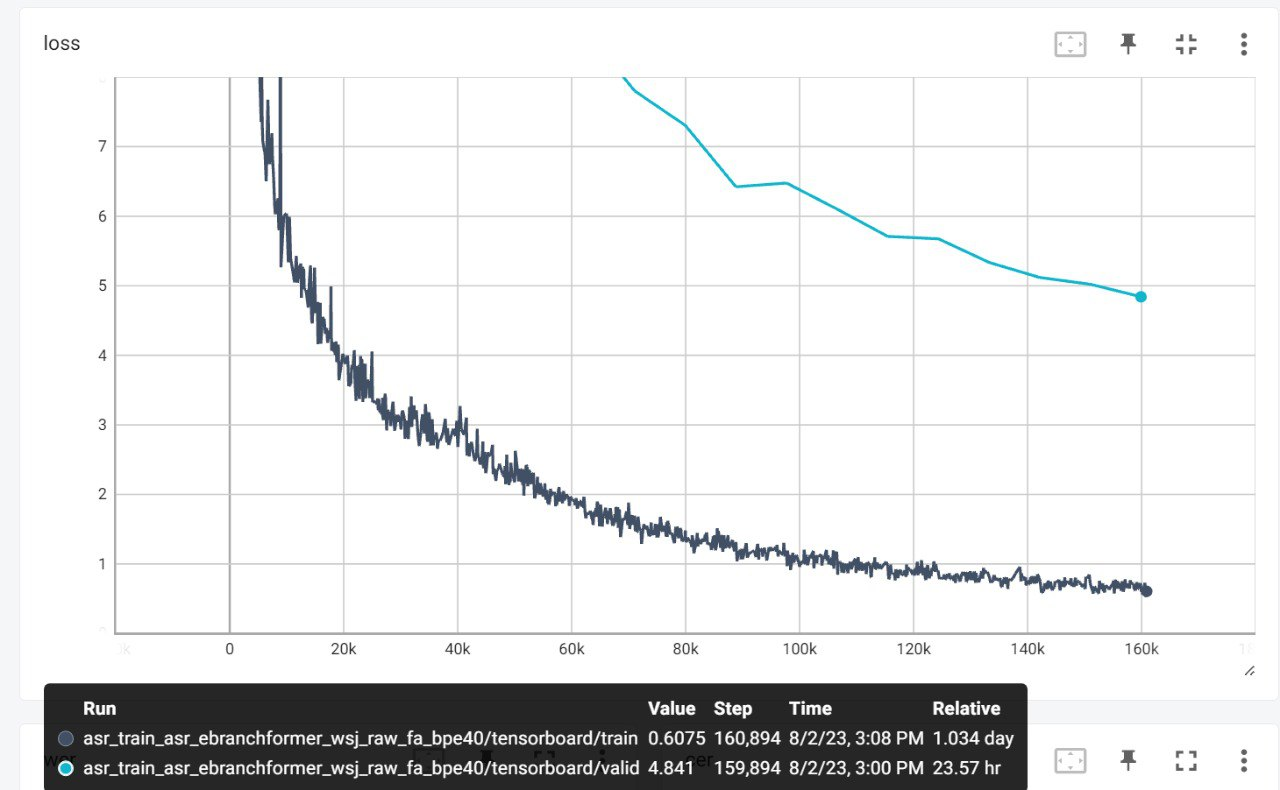
\includegraphics[width=1.1\linewidth, 
                height=0.25\textheight]
                {Images/Chapter3/train3.jpg}
			\caption{مقدار تابع هزینه مدل}
			\label{Cost}
		\end{subfigure}\hfil % <-- added
		\begin{subfigure}{0.5\textwidth}
			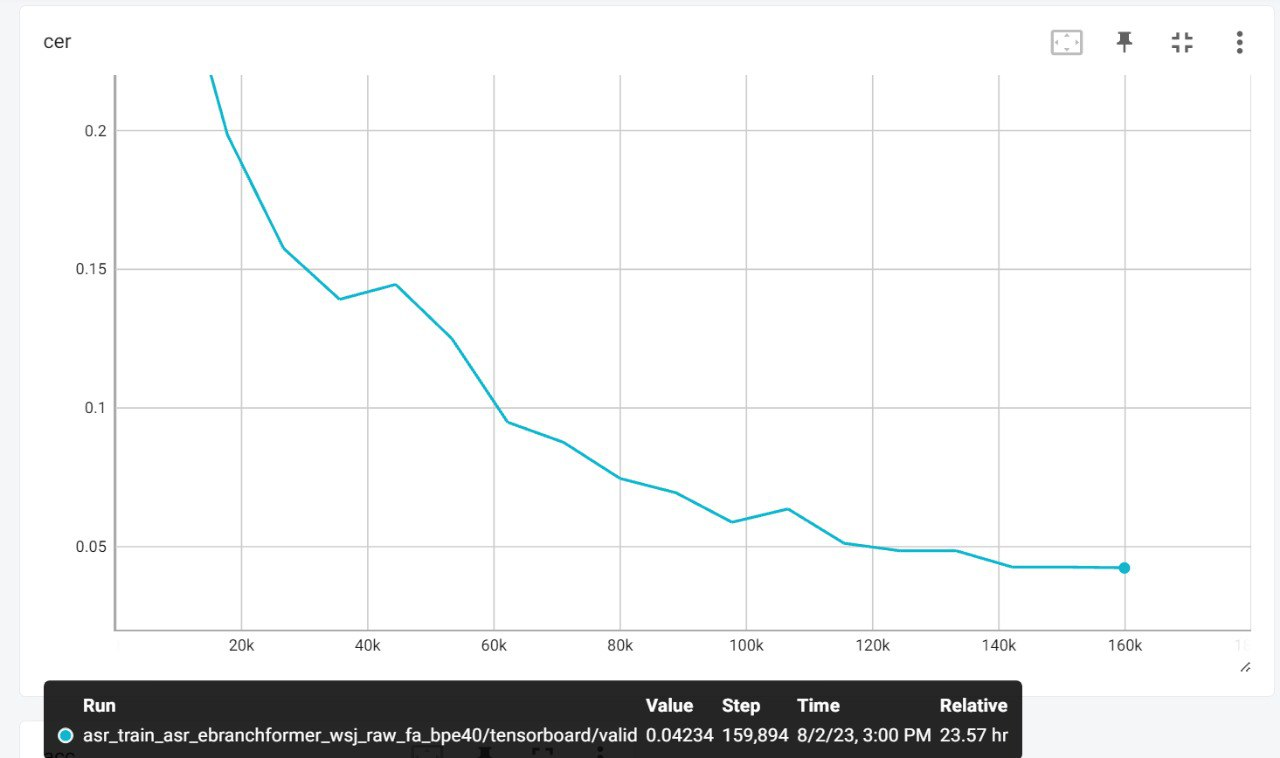
\includegraphics[width=1.1\linewidth, 
                height=0.25\textheight]
                {Images/Chapter3/train4.jpg}
			\caption{مقدار خطای حروف مدل}
			\label{CER}
		\end{subfigure}\hfil % <-- added
		\begin{subfigure}{0.5\textwidth}
			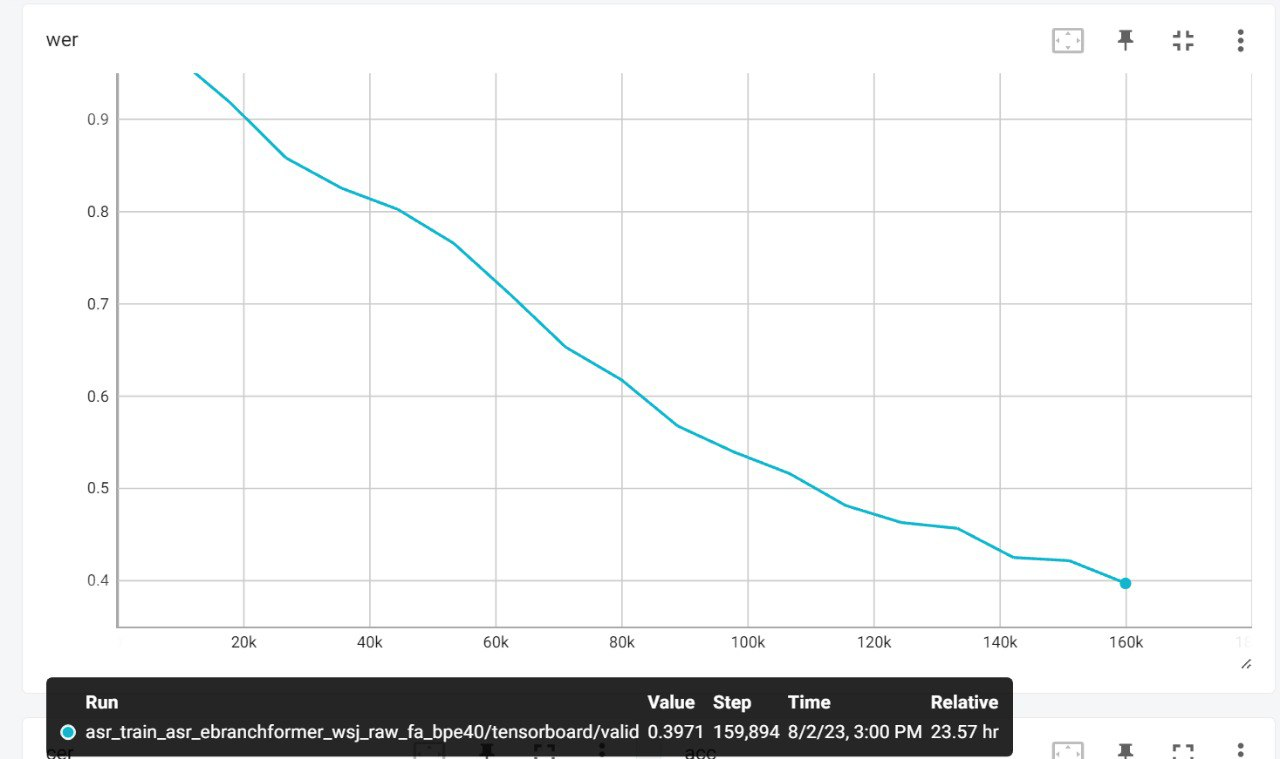
\includegraphics[width=1.1\linewidth, 
                height=0.25\textheight]
                {Images/Chapter3/train5.jpg}
			\caption{مقدار خطای کلمه مدل}
			\label{WER}
		\end{subfigure}
		\caption{تصاویر مربوط به روند آموزش مدل صوت شنانسی بازشناسی گفتار 
  فارسی. این تصاویر خروجی تنسوربرد می‌باشند.}
		\label{fig:train}
\end{figure}

شکل \ref{fig:train} روند آموزش مدل صوت شنانسی را نمایش می‌دهد.
این تصاویر با استفاده تنسوربرد\LTRfootnote{Tensor Board} ایجاد شده اند که درک روند آموزش مدل را با تصاویر و گزارشاتی که ارائه می‌کند بسیار راحت می‌کند.\cite{tensorflow2015-whitepaper}
همین طور که از تصاویر مشخص است مدل روند بسیار پایداری در طول آموزش داشته است و خروجی بسیار رضایت بخش می‌باشد. برای نرخ خطای حروف\LTRfootnote{CER: Character Error Rate}
مقدار $0.04$ بر روی دیتای های ولیدیشن\LTRfootnote{Validation}
بدست آمده است.
و همچنین مقدار $0.397$ درصد برای نرخ خطای کلمه\LTRfootnote{WER: Word Error Rate} بدست آمده است.
نرخ خطا کلمه و حروف
از مهمترین متریک های ارزیابی مدل های بازشناسی گفتار می‌باشند که نتایج حاصله با توجه به حجم دادگان و نوع آنها بسیار رضایت بخش می‌باشد.

برای آموزش این مدل همان طور که مقاله ای-برانچفرمر تاکید کرده است \cite{kim2022ebranchformer}
از دستورعمل های پیش فرض 
یی-اس-پی نت
استفاده شده است اما در مواردی که نیاز به تغییر جزئیات به منظور مناسب سازی برای زبان فارسی بوده است کد ها به صورت دستی تغییر داده شده‌اند. در با توجه به نبود هیچ دوره و آموشی در مورد آموزش دادن مدل زبانی با 
یی-اس-پی نت
وجود نداشت به استفاده از مدل صوت شنانسی اکتفا شده اما در مراحل بعد یک مدل زبانی برای مدل آموزش داده شده است که خروجی آن را بهبود ببخشد.

\section{بررسی خروجی و رفع ایرادات}

همانطور که پیشتر اشاره شد در بازشناسی گفتار یک مدل زبانی به کنار یک مدل صوت شنانسی قرار می‌گیرد که درک گفتار و نوشتار آن به بهترین حالت ممکن صورت بپذیرد با این حال می‌توان از مدل صوت شنانسی به تنهایی برای این منظور استفاده کرد که باعث کاهش دقت زبانی گفتار رونویسی شده می‌شود. با این حال در این مرحله مدل صوت شنانسی را بر روی دادگان تست دیکد کردم تا خروجی تست آن را بررسی کینم.

\begin{figure}[H]
  \centering
  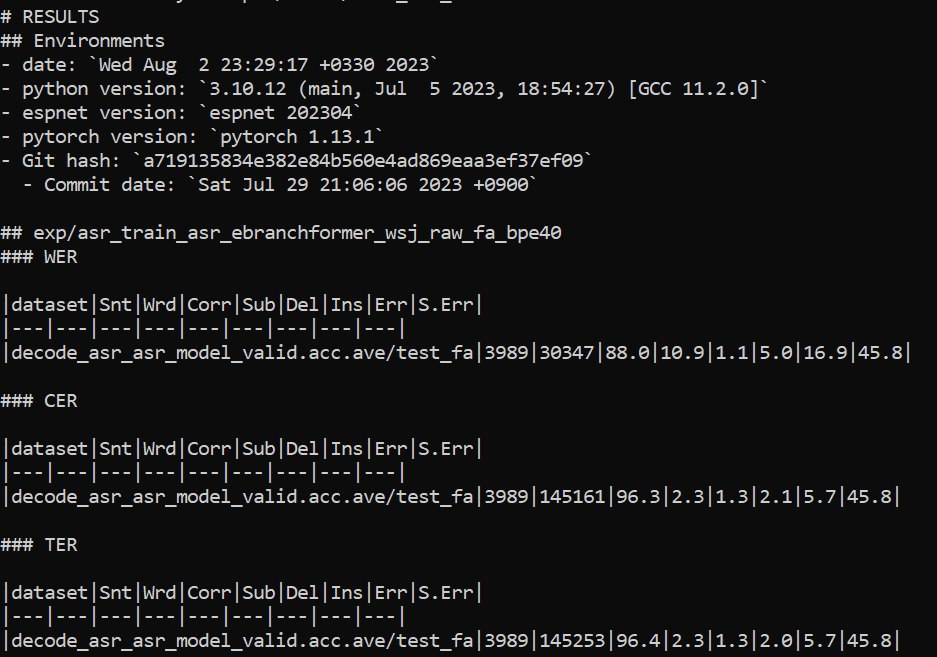
\includegraphics[width=1\textwidth,height=7cm]{Images/Chapter3/decode.jpeg}
  \caption{
  نتایج دیکد مدل صوت شنانسی بدون مدل زبانی بر روی دادگان تست کامن ویس
  }
  \label{fig:decode1}
\end{figure}

شکل \ref{fig:decode1} خروجی مدل را بر روی دادگان تست کامل ویس نشان می‌دهد.
مقدار نرخ خطای کلمه $16.9$ برای کاربرد های امروز نرخ بالایی است اگرچه وجود یک مدل زبانی کنار مدل صوت شنانسی می‌تواند این نرخ خطا را تا نصف کاهش دهد با این حال در کاربرد های امروزی این نرخ بالایی می‌باشد.

در ادامه روند آموزش توسط ارشد پروژه مورد بررسی قرار گرفت و تعدادی از ایرادات که مرتبه اول آموزش مرتکب شدم شناسایی شد و برای اصلاح آنها تلاش شد. در ادامه به تعدادی از مهم ترین این خطاها و راهکار هایی که برای اصلاح آنها انجام دادم اشاره خواهد شد؛ پس از اصلاح این ایرادات مدل دوباره آموزش داده شد و نتایج بسیار ارزشمندی حاصل شد.
\subsection{اشتباه در انتخاب درست تعداد مجموعه توکن ها}
بعد از بررسی هایی که توسط تیم انجام شد یکی از اشتباهات من در طول آموزش انتخاب اشتباه تعداد اعضای مجموعه توکن ها بود.
در ابزار یی-اس-پی نت استیج پنجم آموزش در بازشناسی گفتار باید مجموعه توکن های مشخص شود. زمانی که از مدل های
توجه
استفاده می‌شود باید توکن لیستی از حروف زبان فارسی ایجاد شود که مدل هر آوایی را به یک توکن متناظر\LTRfootnote{Map} کند و رونویسی زبان فارسی را یادبگیرد.
این کار می‌تواند به سه نوع در یی-اس-پی نت انجام شود.

\begin{enumerate}

  \item بر اساس حروف: در این حالت مجموعه توکن ها حروف های زبان فارسی می‌باشد

  \item بر اساس کلمات: در این حالت مجموعه توکن ها بر اساس کلمات زبان فارسی می‌باشد

  \item براساس مدل \texttt{\raggedright bpe}: در حالت ترکیبی از کلمات و حروف ها برای زبان فارسی ایجاد می‌شود.

\end{enumerate}

برای زبان فارسی با توجه به تکراری بودن بعضی از ترکیبات کلمات در اکثر جملات فارسی بهتر است که از 
\verb|bpe|
استفاده شود.
برای استفاده از این نوع ایجاد کننده توکن باید به ابزار یه سری اطلاعات بدهیم. برای مثال باید تعداد اعضای مجموعه توکن ها را با مشخص کردن مقدار متغییر 
\verb|nbpe|
انجام دهیم. برای مثال اگر مقدار این متغییر را 150 بگذاریم خود ابزار ای-ای-پی نت برای ما لیستی از 150 توکن (که تعدادی از آنها حروف و تعدادی دیگر کلمه می‌باشند) ایجاد می‌کند و آن را در یک فایل به نام \verb|tokens.txt|
ذخیره می‌کند. این فایل بعدا توسط مدل برای آموزش استفاده می‌شود.

من در بار اول آموزش اشتباها مقدار
\verb|nbpe|
را 40 گذاشتم ولی در واقع مقدار استاندارد آن 150 می‌باشد و این کار باعث شده بود بعضی از حروف مانند "ژ" در مجموعه توکن های نباشد. این امر باعث کاهش شدید دقت مدل  شده بود و پس از اصلاح آموزش را دوباره آغاز کردم و نتایج جدید بدست آمد.
\begin{figure}[H]
		\centering % <-- added
		\begin{subfigure}{0.5\textwidth}
			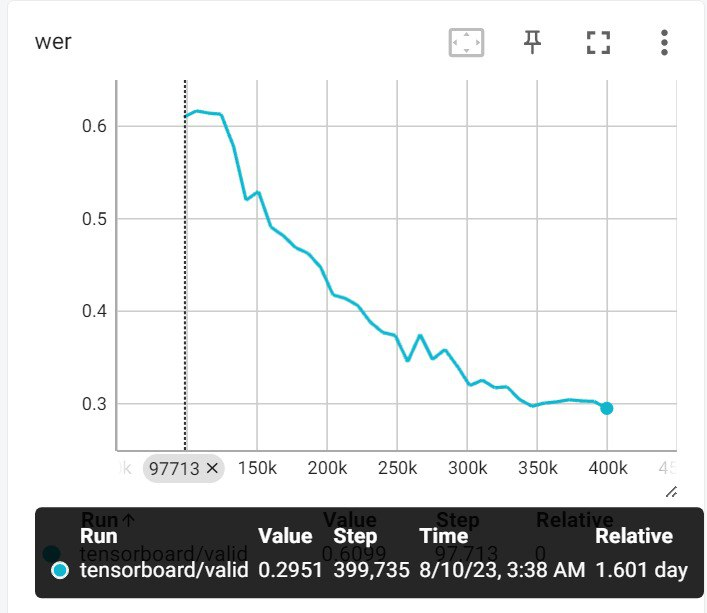
\includegraphics[width=1.1\linewidth, height=0.25\textheight]{Images/Chapter3/train1501.jpg}
			\caption{نرخ خطا  کلمه بر روی ولیدیشن}
			\label{f1}
		\end{subfigure}\hfil % <-- added
		\begin{subfigure}{0.5\textwidth}
			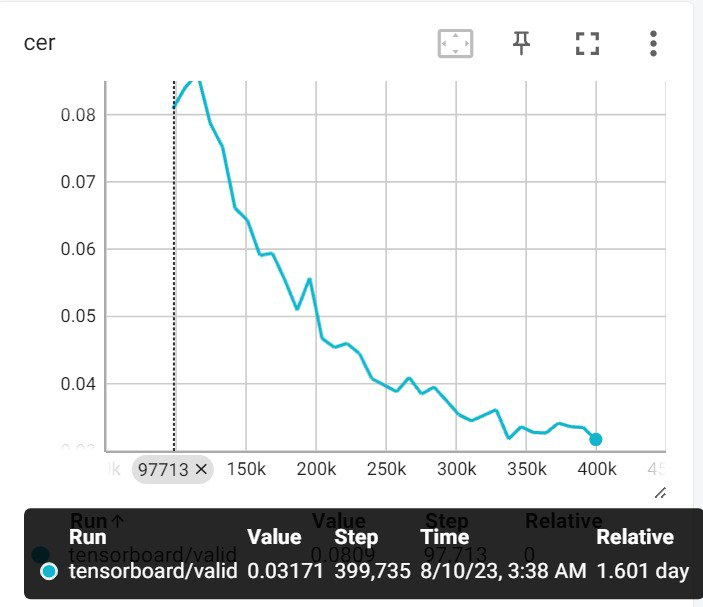
\includegraphics[width=1.1\linewidth, height=0.25\textheight]{Images/Chapter3/train1502.jpg}
			\caption{نرخ خطا حروف بر روی ولیدیشن}
			\label{f2}
		\end{subfigure}\hfil % <-- added
		\label{fig:train150}
            \caption{نمودار های روند آموزش و خروجی آنها بر روی مجموعه ارزیابی با 150 توکن}
\end{figure}
همین طور که در تصویر \ref{f2} و \ref{f1}مشخص است بعد از اعمال تغییرات متریک های مدل بر روی ولیدیشن بهتر شده است. همچنین بر روی تست ست هم خروجی دوبرابر بهتر شده و نرخ خطای کلمات به 8 درصد رسیده است.

\subsection{عدم استفاده از کل داده ها}
با توجه به اینکه روند پیش پردازش داده ها بر روی 
\verb|CPU|
انجام می‌شود و باید تمام فایل های صوتی تغییر فرمت داده شوند من نتوانستم در اولین مرتبه آموزش از کل داده ها استفاده کنم زیرا پیش پردازش کل داده ها روی آن سرور بسیار ارزشمند بود و از بخشی از داده های استفاده کردم. تعداد کم داده ها باعث کاهش دقت مدل شده است و در آموزش جدید از یک سرور با 
\verb|CPU|
قدرتمند تر استفاده شد و خروجی ها بسیار بهبود یافت.

\subsection{عدم استفاده از مدل زبانی}
همانطور که گفته شده برای بهرمندی از بهترین حالت ممکن خروجی باید مدل صوت شنانسی و زبانی کنار هم آموزش داده شوند و استفاده شوند. به همین منظور در این مرحله داده های یک مدل زبانی ترانسفرمری (که در نقش دیکدر در بازشناسی گفتار استفاده می‌شود) بر روی دادگان کامن ویس فارسی آموزش داده شد.آموزش این مدل نصف روز زمان برد. و در نهایت مدل نهای ( که شامل مدل صوت شناسی و زبانی است) بر روی دادگان تست کامن ویس فارسی دیکد شده‌اند و نتایج زیر حاصل شده‌اند.

\begin{figure}[H]
  \centering
  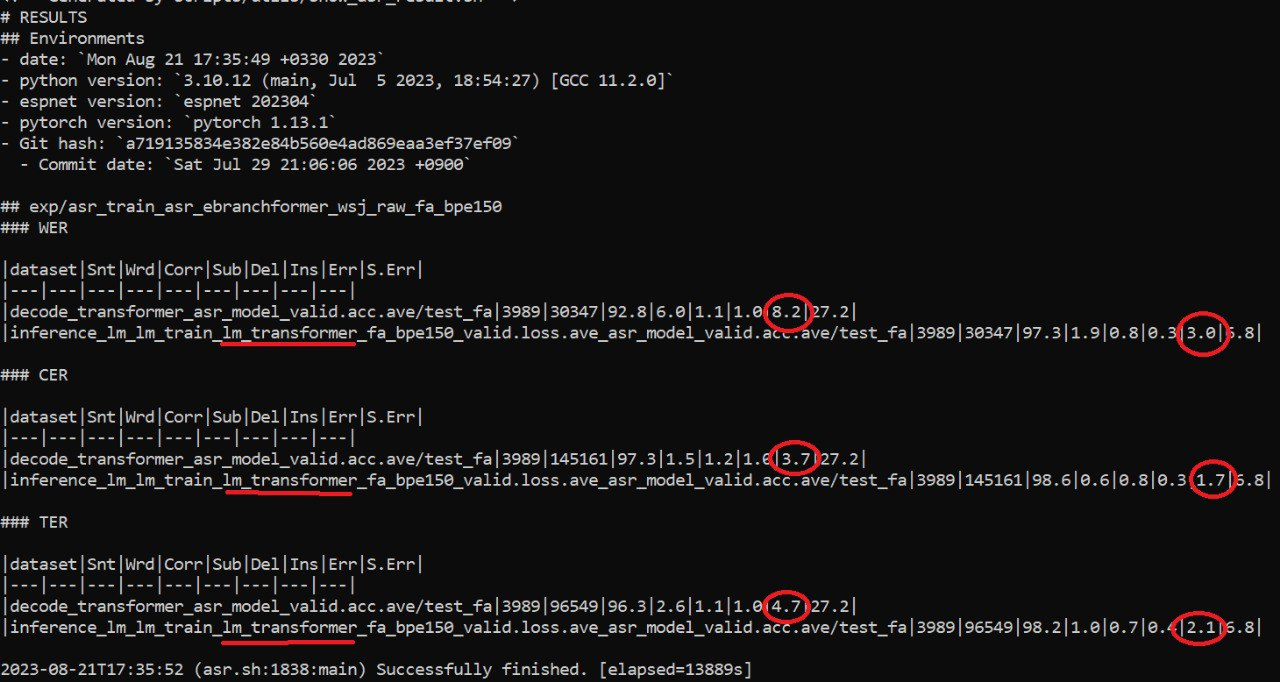
\includegraphics[width=1\textwidth,height=7cm]{Images/Chapter3/decode_best.jpeg}
  \caption{
  نتایج دیکد مدل صوت شنانسی به همراه مدل زبانی بر روی دادگان تست کامن ویس فارسی
  }
  \label{fig:decode_best}
\end{figure}

نتایجی که تصویر \ref{fig:decode_best}
نمایش می‌دهد بسیار عالی و رضایت بخش است. من موفق شدم به نرخ خطای 3 درصد در دادگان تست کامن ویس برسم که این نتیجه در کاربرد فعلی بازشناسی گفتار بسیار عالی می‌باشد. بعد از رسیدن به این نتیاج عالی خروجی مدل در یک جلسه خدمت دکتر صامتی و بقیه اعضای آزمایشگاه نمایش داده شد و مورد قدردانی و تشویق همه اعضا قرار گرفت.

در مرحله بعد کار باید مدل بر روی سرورها پیاده سازی شود که جزئیات مربوط به آن در بخش بعدی بیان خواهد شد.

\section{فراگیری مباحث مورد نیاز برای پیاده سازی بر روی سرور}

در این مرحله کار باید مدل ساخته شده بر روی یک سرور پیاده سازی شود تا بتوان از آن به عنوان یک سرویس جدید برای شرکت استفاده کرد. برای مرحله اول ابتدا باید یک نمونه ساده پیاده سازی شود تا خروجی کار و سرعت عملکرد آن بررسی شود. در ادامه به بررسی چند روش برای پیاده سازی مدل بر روی بک‌اند سرور پرداختم که در نهایت به این نتیجه رسیدم که استفاده از فریم ورک گرادیو\LTRfootnote{Gradio} آسان ترین و سریع ترین راه پیاده سازی مدل های هوش مصنوعی بر روی بک‌اند سرور می‌باشد.\LTRfootnote{ \url{https://github.com/gradio-app/gradio}}


گرادیو
یک کتابخانه پایتون منبع باز است که برای ساخت دموهای یادگیری ماشین و علوم داده و برنامه های کاربردی وب استفاده می شود.
با 
گرادیو
، می توانید به سرعت یک رابط کاربری زیبا در اطراف مدل های یادگیری ماشین یا گردش کار علم داده خود ایجاد کنید و به افراد اجازه دهید با کشیدن و رها کردن در تصاویر خود، چسباندن متن، ضبط صدای خود و تعامل با آن، آن را امتحان کنند.\cite{abid2019gradio}

\section{پیاده سازی بر روی سرور}
در این مرحله از پروژه من اقدام به پیاده سازی مدل بر روی گرادیو کردم. یکی از بزرگترین چالش های این بخش فهمیدن این مسئله بود که چگونه می‌توانیم از مدل آموزش دیده در گرادیو استفاده کنم. با نبود هیچ آموزش و داکیومنتشن در این رابطه من مجبور شدم که دوباره تمام کد های یی-اس-پی نت را بررسی کنم تا در نهایت موفق به پیدا کردن و استفاده از فایل های مربوط به این زمینه در یی-اس-پی نت شدم.
گرادیو را می‌توان به راحتی در هر سروری پیاده سازی کرد ولی برای استفاده عمومی باید سرور قابلیت هاستینگ را داشته باشد. به همین منظور از سرور های هاگینگ فیس\LTRfootnote{Hugging Face} برای پیاده سازی مدل  استفاده شده است.\LTRfootnote{\url{https://github.com/huggingface} , \url{https://huggingface.co/}}

هاگینگ فیس یک شرکت فرانسوی-آمریکایی است که ابزارهایی را برای ساخت برنامه های کاربردی با استفاده از یادگیری ماشین، مستقر در شهر نیویورک توسعه می دهد. این به خاطر کتابخانه ترانسفورماتورهای خود که برای برنامه های کاربردی پردازش زبان طبیعی ساخته شده است و پلتفرم آن که به کاربران اجازه می دهد مدل ها و مجموعه داده های یادگیری ماشین را به اشتراک بگذارند و کار خود را در یک فضا به نمایش بگذارند قابل توجه است.\cite{wolf2020huggingfaces}

بعد از یادگیری کار با هاگینگ فیس و گرادیو موفق شدم نسخه اولیه نرم سرویسی باز شناسی گفتار فارسی را پیاده سازی کنیم. برای دسترسی به این نرم افزار بررسی آن کافی است بر روی این \href{https://huggingface.co/spaces/parsa-mhmdi/persian-asr}{لینک} کلیک کنید.
ر این نرم افزار امکان ضبط فایل صدا و همچینین ارسال فایل صوتی وجود دارد و پس از چند ثانیه پردازش نرم افزار متن گفته شده در فایل صوتی را بازنویسی می‌کند.\LTRfootnote{ \url{https://huggingface.co/spaces/parsa-mhmdi/persian-asr}}
با تمام تلاش های صورت گرفته این نرم افزار همچنان در مرحله توسعه می‌باشد و هنوز آماده کار های تجاری نشده است برای کار های حرفه ای همچنان به کار های بیشتر نیاز دارد. با توجه به اینکه سرور های رایگان هاگینگ فیس فقط اجازه استفاده از
\verb|CPU|
می‌دهد ممکن زمان پردازش مقداری طولانی تر از \verb|GPU|
باشد.

\begin{figure}[H]
  \centering
  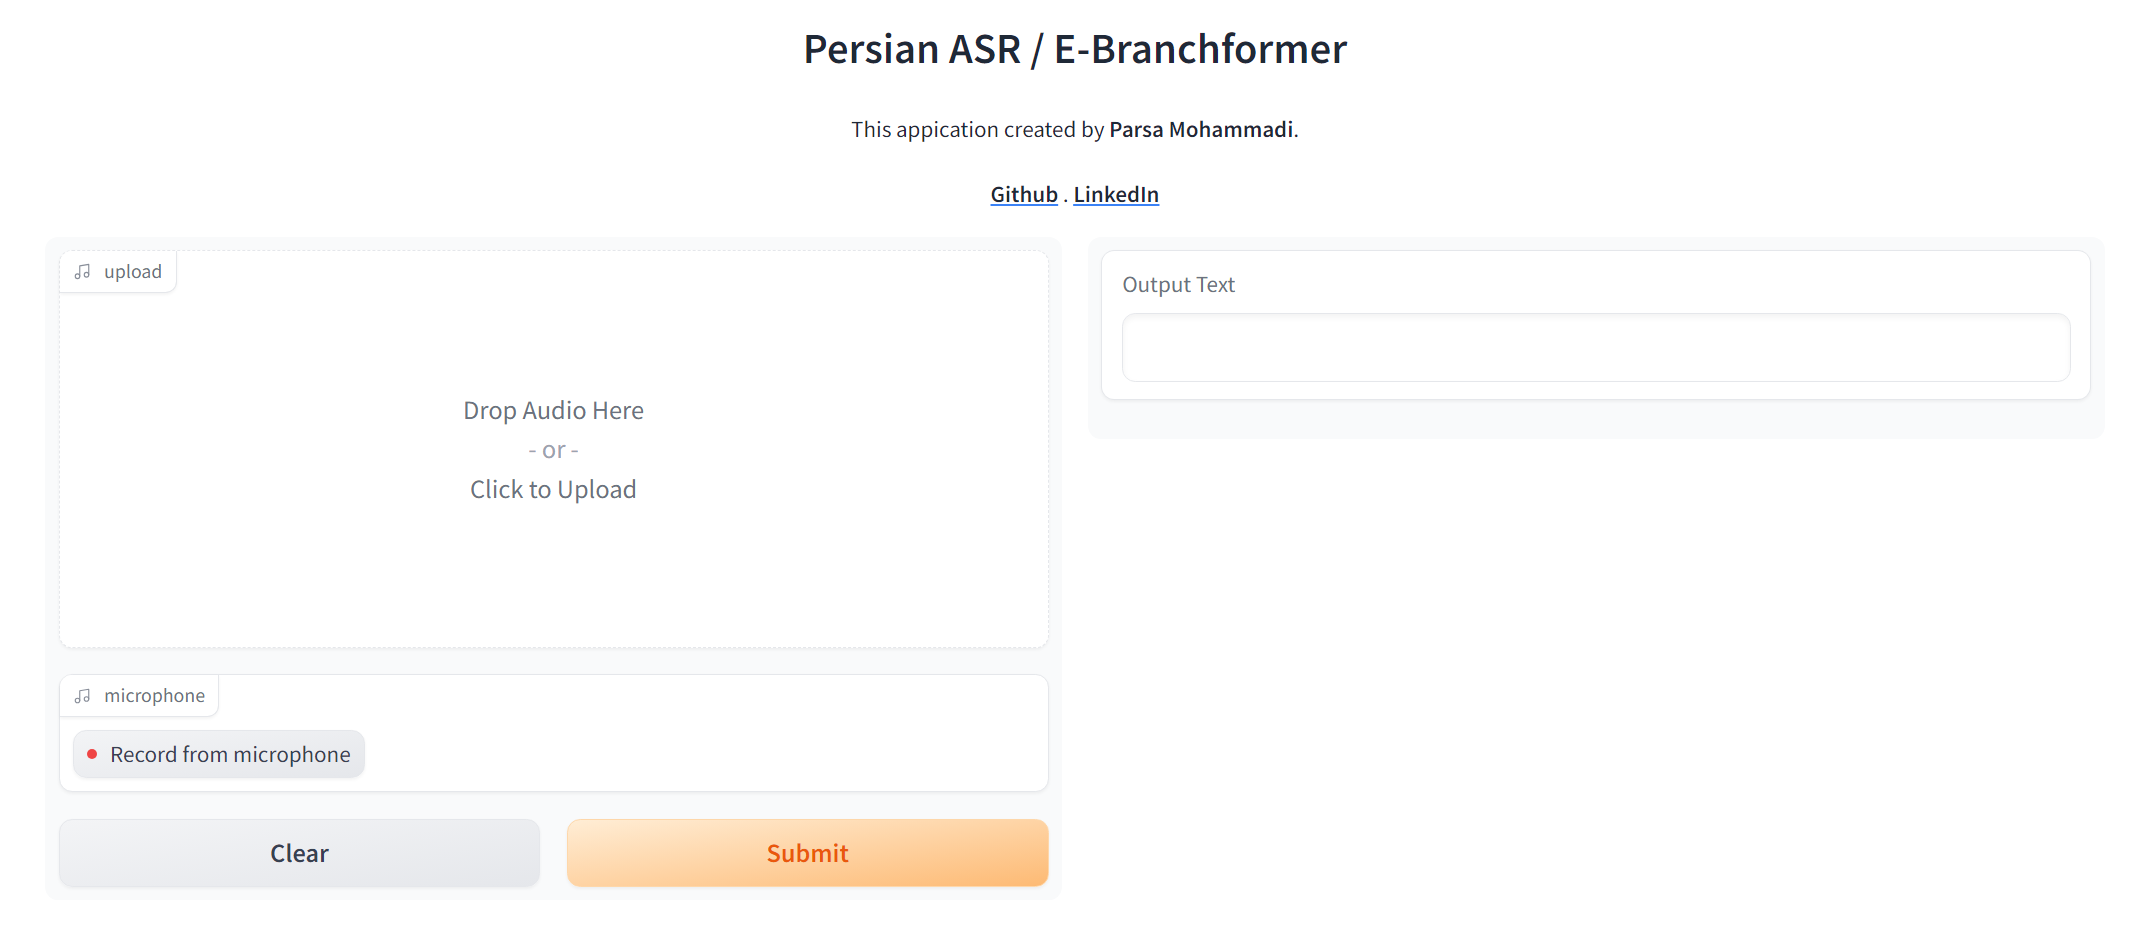
\includegraphics[width=1\textwidth,height=7cm]{Images/Chapter3/UI.png}
  \caption{
  تصویر رابط کاربری نرم افزار بازشناسی گفتار فارسی 
  }
  \label{fig:UI}
\end{figure}

\section{مستندسازی و ارائه خروجی}
در نهایت کار خلاصه از تمام انجام شده و نتایج حاصل شده مستند سازی شده و در جلسه آزماشیگاه ارئه شد. دکتر صامتی ضمن قدردانی پیشنهاد پیاده سازی این مدل بازشناسی گفتار برای زبان عربی را دادند که در صورت ادامه همکاری با شرکت این پروژه برای کارفرمای مربوطه انجام شود. در ادامه تمام کد ها گزاش ها و مدل های آموزش داده شده خدمت شرکت تسلیم شد و بر روی ریپازیتوری کارآموزش قرار گرفت.

بعد از اتمام این تجربه دلنشین و بسیار آموزنده کارآموزی نامه های مربوط به گذراندن 240 ساعت کارآموزی با امضای مدیرعامل شرکت دریافت شد و یک لوح تقدیر به من داده شد. تمام این مدارک در انتهای این گزارش کارآموزی پیوست شده است.










